\chapter{State of the art und Grundlagen}
Mehrere Möglichkeiten
Verkehrszentrale -- trotzdem gibt es manuell geschaltete Ampeln\\
\gls{V2X}- Kommunikation
\section{Einleitung}
Die Verkehrsstrategie des Senats sieht vor, dass das Radfahren bis zum Jahr 2025 20 Prozent des Gesamtverkehrs ausmachen soll. (J.Anker, Berliner Morgenpost, am 6.06.2014)
"Wir brauchen eine intelligente Konstruktion, die alle Verkehrsarten verbindet", sagte Stadtentwicklungssenator Michael Müller (SPD).\\
Für Autos gibt es bereits funktionierende Apps wie EnLighten und SignalGuru, aber auch eingebaute Systeme im Autocomputer von Audi und Toyota, welche anstreben den Verkehr elektronisch optimieren.
% ### Auto ###
\section{Ampel-Informationssysteme im Auto}
\subsection{Toyota}
Toyotas System erfordert eine spezielle Infrastruktur an Kreuzungen, die Installation von Infrarot-Sendern, die mit dem Toyota-GPS kommunizieren. An roter Ampel wird der Fahrer über die verbleibende Wartezeit informiert. Andere Autohersteller wie BMW, Volvo und Volkswagen kooperieren in diesem Forschungsprojekt, mit dem Forschungziel die Sicherheit an Kreuzungen zu verbessern. Im Auto installierte Sensoren kommunizieren mit Kameras und Scanner in der Ampel. \\
Allerdings funktioniert das System nur mit dem ambitionierten Ziel, wenn alle Autohersteller zusammenarbeiten und sich auf den gleichen Standard einigen.
\subsection{Audi}
Audi fragt über das Internet die Daten aus dem ‘area’s central traffic computer’, über die automatisch geschalteten Ampeln an. Damit berechnet das System die Geschwindigkeit, die man benötigt, um so viele grüne Ampeln wie möglich zu passieren.\\
\subsection{Projekt Wolfsburg}
\subsection{Projekt Travolution}
% ### Apps ###
\section{Mobile Ampel-Informationssysteme}
Für den Einsatz in Kraftfahrzeugen stehen sowohl für Android als auch für's iPhone diverse Apps zum Download bereit. 
\subsection{EnLighten}
EnLighten erkennt rote Ampeln und visualisiert die Dauer dieser Phase.  
EnLighten nutzt \gls{GPS} zur Lokalisierung des Autos und verwendet die \gls{V2R}-Kommunikation zu Ampelphasenprognose.
\begin{figure}[h]
    \centering
    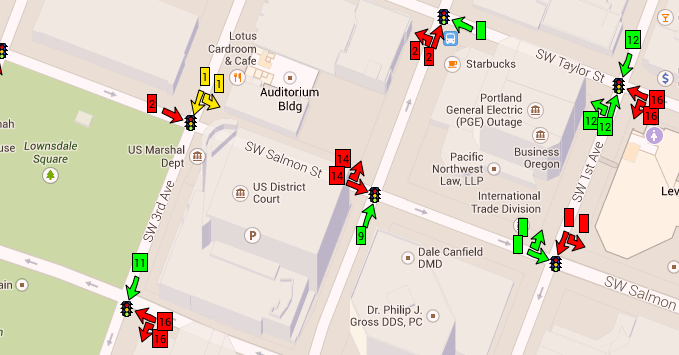
\includegraphics[scale=0.5]{EnLighten}
    \label{fig:Ampelsignalstatus}
    \caption[Echtzeit Ampelsignalstatus]{Schnappschuss der Echtzeit Ampelsignalstatusprognose in Portland}
\end{figure}
Hierbei verbindet sich die App über \gls{DSRC} mit den Lichtsignalanlagen und beachtet dabei Komponenten wie die Höchstgeschwindigkeit, Fahrtrichtung und Tageszeit.
Die Installation der \gls{DSRC}-Hardware an den Komponenten ist sehr aufändig und teuer, weswegen EnLighten erst in einigen amerikanischen Städten funktionstüchtig ist.
\subsection{SignalGuru}
Die App SignalGuru errechnet über die Smartphones vieler Nutzer - welche miteinander kommunizieren -  die Wahrscheinlichkeit, wann eine Ampel grün wird und wie das eigene Fahrverhalten entsprechend anzupassen ist. Hierbei muss die eingebaute Kamera durch die Windschutzscheibe die Ampel registrieren. Bei Testläufen im Straßenverkehr vielen die Ergebnise bei statisch geschalteten Ampeln deutlich besser aus als bei angepassten Ampelschaltungen \footnote{Vgl. \cite{SignalGuru}} 
Die Smartphones kommunizieren miteinander und teilen sich die Dauer der Ampelphasen mit. So entsteht mit der Zeit ein recht genaues Muster über die Schaltpläne der Ampeln. Daraus wiederum lässt sich vorausberechnen, welche Phase eine Ampel zeigt.
http://www.golem.de/1108/86013.html
\begin{figure}[h]
    \centering
    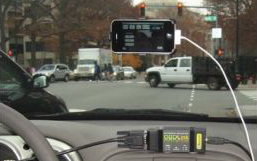
\includegraphics[scale=0.8]{SignalGuru}
    \caption[Signal Guru]{Signal Guru App muss in der Lage sein die Ampel zu 'sehen'.  \cite{SignalGuruPaper}}
    \label{fig:AbbSignalGuru}
\end{figure}
Ob das auch in Deutschland funktioniert ist schwer zu sagen, da die Ampeln hierzulande so gesetzt sind, dass das Smartphone in der Pole-Position die Ampel evtl. nicht erfassen kann. Dies gilt es in der Entwicklungsarbeit zu testen und gegebenenfalls auszuarbeiten.
\subsection{Ampelmeter}
\subsection{Analyseergebnis}
Diese Beispiele zeigen deutlich, dass die Nachfrage nach Ampel-warnsystemen -- mobil oder statisch -- steigt und auf dem Markt Anklang findet. Der Verkehr ist flüssiger, die Teilnehmer entspannter, die Luft sauberer. AutofahrerInnen sind schon lange nicht mehr allein auf der Straße und so gilt es, dieses erfolgreiche Konzept für alle Verkehrteilnehmer zu erweitern.
% ### Technische Grundlagen ###
\section{Technische Grundlagen}
\subsection{Arduino / Android-App}
\subsubsection{Mobile Sensing}
\textit{Der Beschleunigungssensor ist ein Hardwaresensor, der dazu benutzt wird, Position, Bewegung, Neigung, Erschütterung, Vibration und natürlich Beschleunigung des Gerätes zu messen.Es gibt bis zu 3-Achsen Beschleunigungssensoren, die meistens zum Erkennen der Ausrich-
tung des Smartphones genutzt werden und somit das Display beim Anschauen von Bildern,
Webbrowsern oder Musikplayern in die passende Richtung vom Portrait-Modus (senkrecht)
zum Landscape-Modus (waagrecht) zu drehen. In Kombination mit GPS kann das Smartphone
dank ihm sogar erkennen, welche Art Transportmittel (Fahrrad, Bus, U-Bahn) der Nutzer gerade
benutzt und bestimmte Muster wie z.B. Rennen, Gehen oder Stehen unterscheiden.\\\\
GPS oder Global Positioning System erlaubt dem Smartphone sich selber zu lokalisieren und
den exakten Standpunkt auf der Erde zu bestimmen. Es hilft locationbased\footnote{ortsgebunden} Apps wie z.B Navigation, lokale Suche nach Shops, Restaurants etc. oder soziale Netzwerke wie Facebook oder Foursquare nötige Informationen zu ermitteln. Der Kompass erweitert die Möglichkeiten der Lokalisationsermittlung eines Smartphones. Er bestimmt den Winkel des Geräts relativ zum Nordpol der Erde. Der Kompass besitzt einen Magnet, der mit dem magnetischen Feld der Erde interagiert und sich entsprechend zu einem der Pole ausrichtet. Zusammen mit dem Gyroskop Sensor verbessern GPS und Kompass die Präzision von locationbased Applikationen.Der Gyroskop Sensor bestimmt die Rotations- und Drehgeschwindigkeit des Smartphones auf seinen drei Achsen gegenüber dem Weltkoordinatensystem.}
\subsection{Backend mit nodejs / socket.io und MongoDB}
\subsection{Open-Street-Map}
